\begin{figure*}[h]
  \centering
  \begin{minipage}{0.33\textwidth}
    \centering
    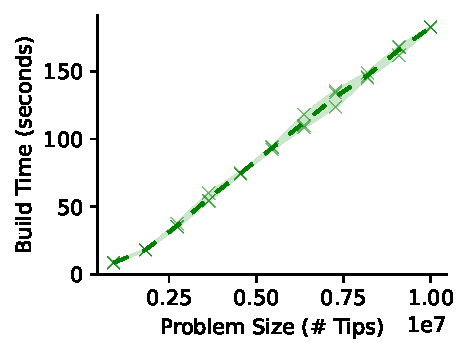
\includegraphics[height=4.3cm]{img/longterm-purifying.pdf}
    \subcaption{Purifying Regime}
    \label{fig:asymptotic:purifying}
  \end{minipage}%
  \begin{minipage}{0.33\textwidth}
    \centering
    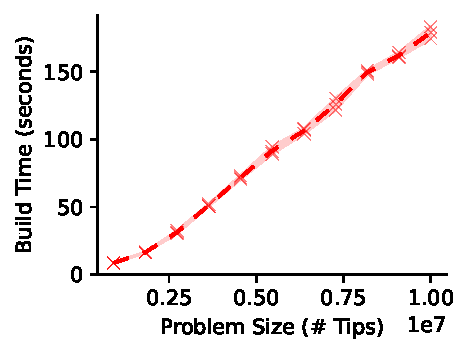
\includegraphics[height=4.3cm,trim={0.7cm 0 0 0},clip]{img/longterm-adaptive.pdf}
    \subcaption{Adaptive Regime}
    \label{fig:asymptotic:adaptive}
  \end{minipage}%
  \begin{minipage}{0.33\textwidth}
    \caption{%
    \textbf{Empirical performance scaling of shortcut table algorithm in microbenchmark trials.}
    \footnotesize
    Panels \ref{fig:asymptotic:purifying} and \ref{fig:asymptotic:adaptive} differ in simulation data source of sampled genomes, with the former exhibiting higher phylogenetic richness.
    Shaded bands are 100\% percentile intervals, with 3 samples taken per problem size.
    Adapted from \citet{singhvi2025scalable}.
}
    \label{fig:asymptotic}
  \end{minipage}
\end{figure*}
